\chapter{序論}
\label{chap:introduction}
\section{背景}

% なぜこの研究が必要だったのか、しっかりした理屈を考えておく。
% 現状どういう問題があるのか
% どういう方法で解決を試みたのか
% 結果として上手く行ったのか、いかなかったのか

近年、スマートフォンなどのモバイルインターネット端末が爆発的に普及し、あらゆる年代の利用者に用いられるようになった。
もはや生活の一部とも言える存在となったスマートフォンだが、私が日常的に使用する中で不便だと感じる点がある。
それはAndroid Widgetを用いた情報の獲得についてである。
Android Widgetを画面に配置しておくと、ユーザが能動的に操作をしなくとも、最新の情報が常に画面に表示されるので情報を効率的に入手することが出来る。

しかし、Android Widgetはいくつかの問題を抱えている。
まずAndroid端末の一つの画面に置くことの出来るAndroid Widgetの数は限られているため、獲得できる情報の種類も限られてしまうという問題である。(図\ref{fig:old_widget})
例えば天気予報を見たければ天気予報のAndroid Widgetを画面に設置し、別の情報が必要であればまた別のAndroid Widgetを設置する必要がある。
Android Widgetの性質上、取得したい情報に付随して不要な情報までもが表示され、それによって画面スペースが埋められてしまうというケースも存在する。
また、自分の取得したい情報に対応したAndroid Widgetが存在しない場合、自らAndroid Widgetを作成する以外の対応策がない。
現状ではAndroid Widgetの作成は多数のスマートフォンユーザにとって技術的なハードルが高く、問題の解決法としては現実的ではない。

本研究では単体で複数の情報を表示することの出来るAndroid Widgetを作成することでこれらの問題の解決を図った。

\begin{figure}[htbp]
  \begin{minipage}{\hsize}
    \begin{center}
      \fbox{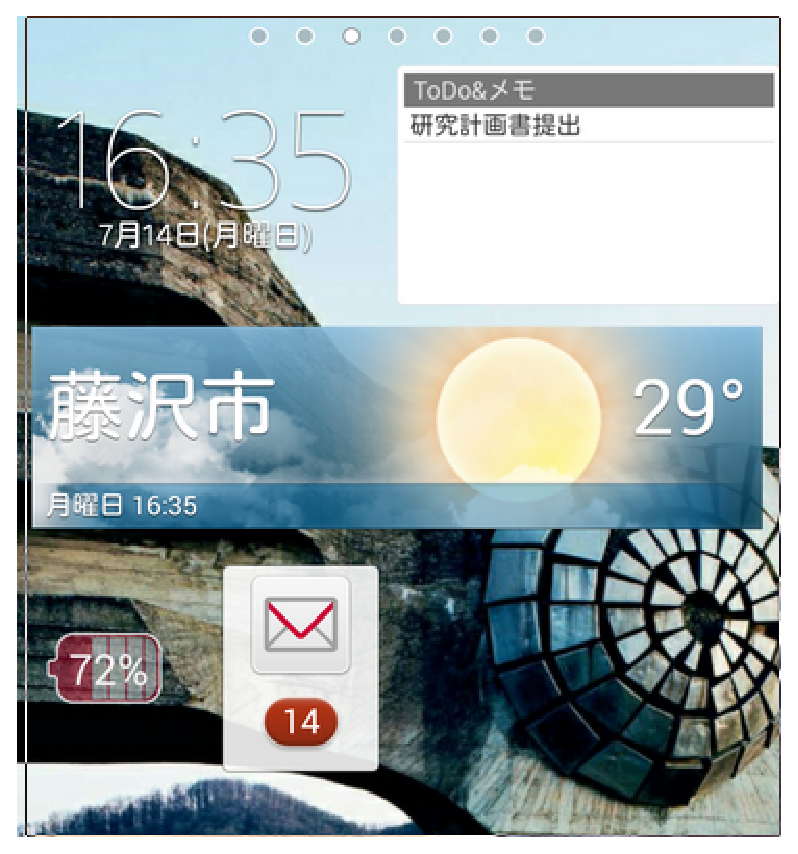
\includegraphics[width=100mm]{image/old_widget.eps}}
    \end{center}
    \caption{現状のAndroid Widgetを使用した画面}
    \label{fig:old_widget}
  \end{minipage}
\end{figure}

\section{目的}
%こんな素敵なことが出来るようになるんだよ。
本研究の目的は、ユーザが必要とする様々な情報をコンパクトに表示するシステム及びインタフェースの実現である。
それによって情報の獲得が容易になり、さらに取得する情報からノイズが減ることになり、ユーザは効率良く価値の高い情報を得ることが出来るようになる。
%また現状ではAndroid Widgetとして表示することの難しい情報の取得が容易になることで、
%そのため、まずはユーザが必要とする可能性のある情報を予め取得し、記録しておくことが必要である。次に記録したデータから、ユーザ自らが取得したいデータを選択できるインタフェースを用意し、そこで選択されたデータをユーザに提供することでユーザが知りたい情報のみを取得・表示できるインタフェースを実現する。

\section{本論文の構成}

第\ref{chap:contents}章では研究内容を説明する。第\ref{chap:prototype}章ではプロトタイプの実装方法を解説する。第\ref{chap:consideration}章では考察を書く。最後に第\ref{chap:conclusion}章にて結論を書き本論文をしめることとする。添付として参考文献を追記する。
